\documentclass{beamer}


\usetheme{default}
\title{Informe de resultados}
\author{Fernando Sanchez Sanchez}

\usepackage{Sweave}
\begin{document}
\Sconcordance{concordance:Proyecto_presentación_FSS.tex:Proyecto_presentación_FSS.Rnw:1 %
7 1 1 0 36 1 1 5 35 1}


\begin{frame}
\frametitle{Presentacion preliminar de resultados}
PROYECTO DE CIENCIA DE DATOS.
Resultados iniciales
\end{frame}

\begin{frame}
\frametitle{Resultados numericos}

\begin{table}[ht]
\centering
\caption{Medias por categoría de maritalb}
\begin{tabular}{|l|c|c|c|}
\hline
maritalb & ppltrst\_media & pplfair\_media & pplhlp\_media \\
\hline
Casado/a & 5.0 & 5.5 & 4.9 \\
Pareja de hecho & 5.9 & 6.3 & 5.5 \\
Separado/a & 4.8 & 5.2 & 4.9 \\
Divorciado/a & 4.8 & 5.4 & 4.7 \\
Viudo/a & 4.4 & 5.1 & 4.6 \\
Soltero/a & 5.1 & 5.5 & 5.0 \\
NA & 4.5 & 5.1 & 4.7 \\
\hline
\end{tabular}
\end{table}


\end{frame}

\begin{frame}
\frametitle{Participantes}




El numero total de participantes en el estudio es \emph{37611}.


\end{frame}

\begin{frame}
\frametitle{Resultados graficos. Pagina 1 del dashboard}
\begin{figure}[ht]
\centering
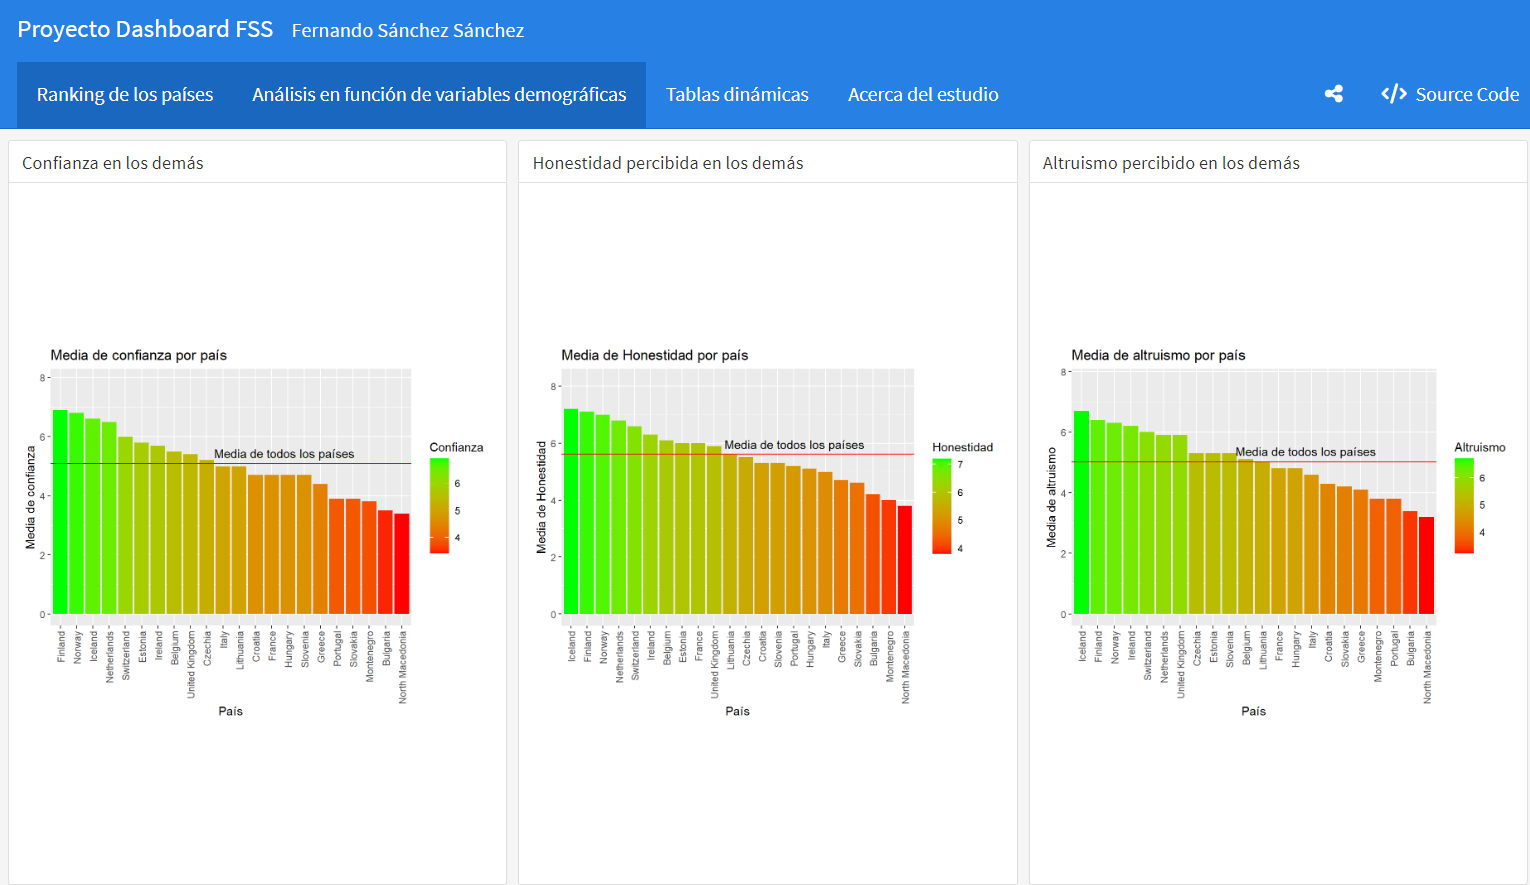
\includegraphics[width=0.8\textwidth]{Figura_1.png}
\caption{Resultados iniciales}
\end{figure}
\end{frame}

\begin{frame}
\frametitle{Resultados graficos. Pagina 2 del dashboard}
\begin{figure}[ht]
\centering
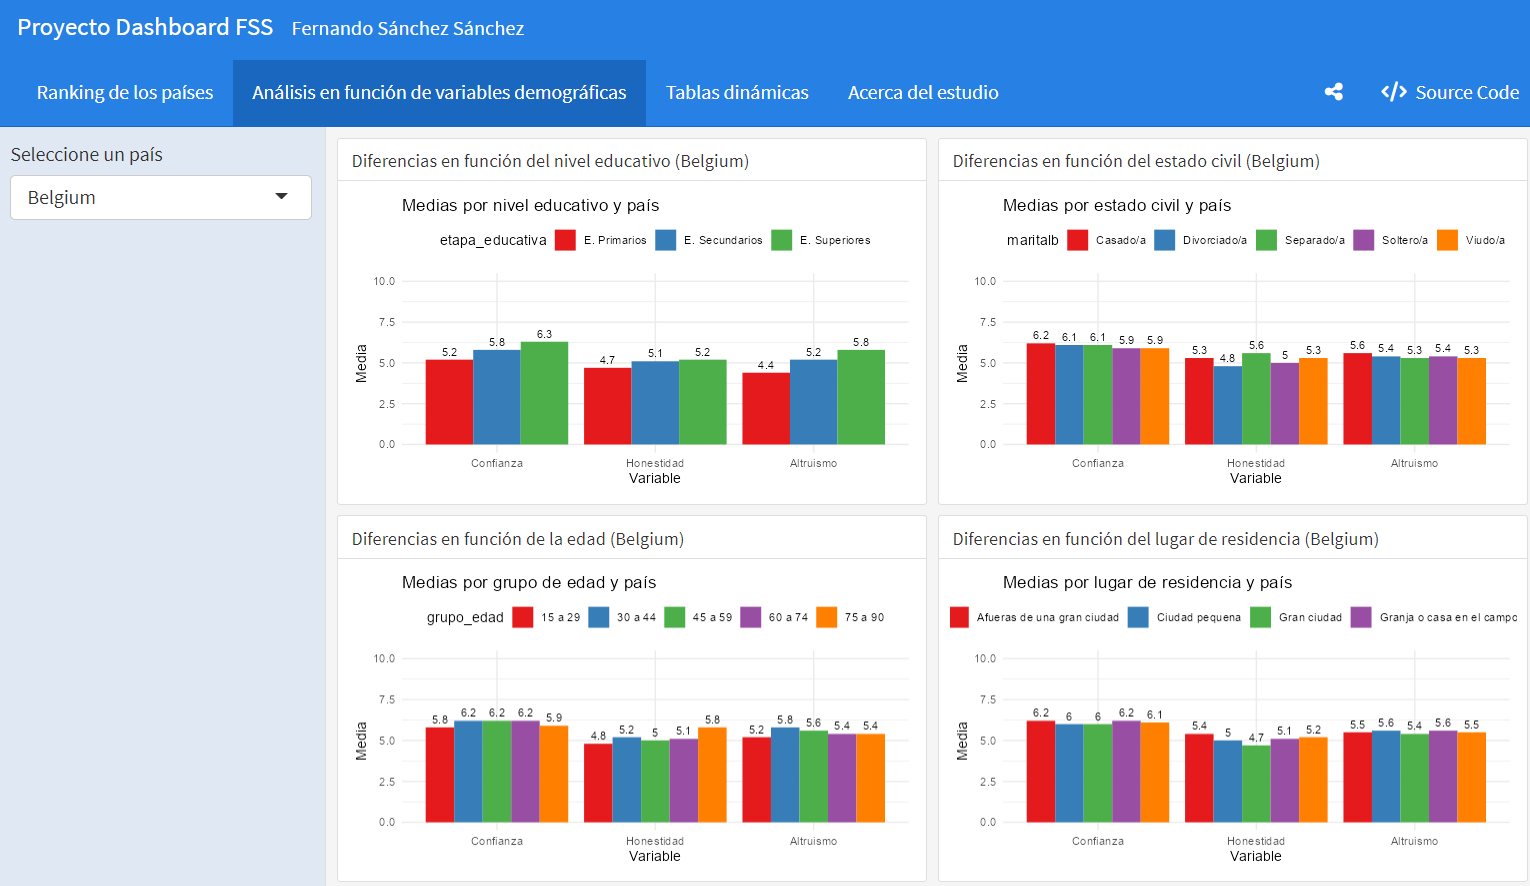
\includegraphics[width=0.8\textwidth]{Figura_2.png}
\caption{Resultados iniciales}
\end{figure}
\end{frame}

\begin{frame}
\frametitle{Resultados graficos. Pagina 3 del dashboard}
\begin{figure}[ht]
\centering
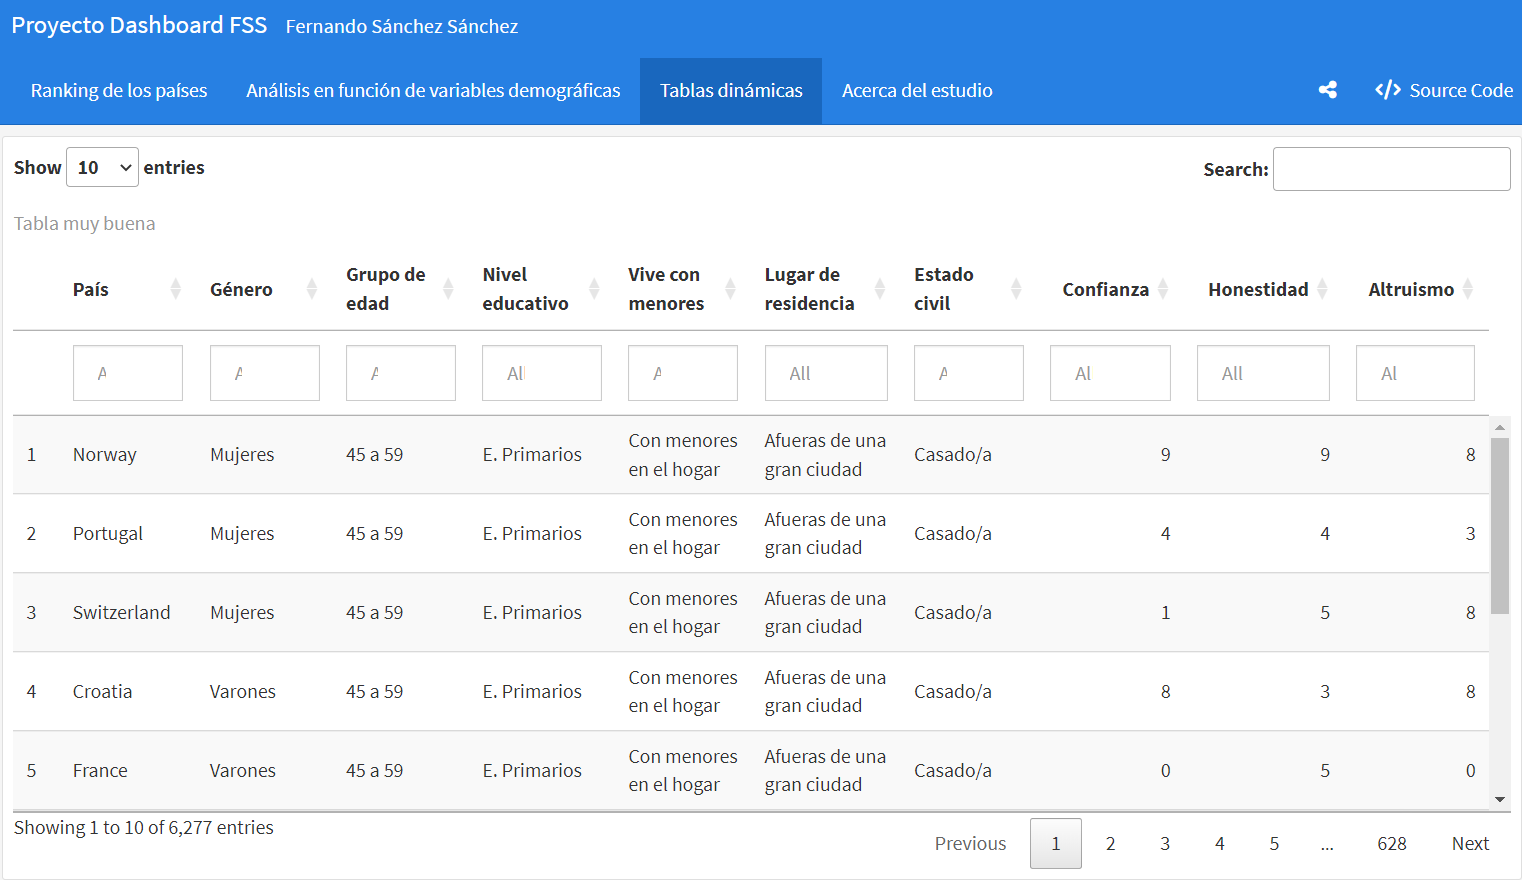
\includegraphics[width=0.8\textwidth]{Figura_3.png}
\caption{Resultados iniciales}
\end{figure}
\end{frame}

\end{document}

